% Print version of the blueprint (pdflatex print.tex).
% The leanblueprint tool supplies its own print.tex and web.tex; this file lets
% the PDF be built without it, by defining the blueprint commands as no-ops.
\documentclass[11pt]{report}
\usepackage[margin=1.1in]{geometry}
\usepackage{amsmath,amssymb,amsthm,mathtools}
\usepackage{graphicx}
\usepackage{pdflscape}
\usepackage[colorlinks=true,linkcolor=blue,urlcolor=blue]{hyperref}
\makeatletter
% \lean and \uses take comma-separated lists; print them so that lines can break
\newcommand{\lean}[1]{\par\noindent{\footnotesize\textsf{Lean:}\ \raggedright
  \@for\@n:=#1\do{\texttt{\expandafter\detokenize\expandafter{\@n}}\ \allowbreak}\par}}
\newcommand{\leanok}{}
\newcommand{\uses}[1]{\par\noindent{\footnotesize\textsf{Uses:}\ \raggedright
  \@for\@u:=#1\do{\ref{\@u}\ \allowbreak}\par}}
\makeatother
\theoremstyle{plain}
\newtheorem{theorem}{Theorem}[chapter]
\newtheorem{lemma}[theorem]{Lemma}
\theoremstyle{definition}
\newtheorem{definition}[theorem]{Definition}
% Macros shared by the print and web versions of the blueprint.
\newcommand{\R}{\mathbb{R}}
\newcommand{\N}{\mathbb{N}}
\newcommand{\eps}{\varepsilon}
\newcommand{\dlap}{\Delta}
\newcommand{\pnlap}{\Delta_p^{N}}
\newcommand{\inflap}{\Delta_\infty^{N}}
\newcommand{\Op}{T_\eps}
\newcommand{\avgint}{\fint}
\newcommand{\fint}{\mathop{\mathrlap{\,\rule[0.62ex]{0.62em}{0.5pt}}\int}}
\newcommand{\abs}[1]{\left\lvert #1\right\rvert}
\newcommand{\norm}[1]{\left\lVert #1\right\rVert}
\newcommand{\usc}{\operatorname{usc}}
\newcommand{\lsc}{\operatorname{lsc}}
\newcommand{\viscF}{\mathcal{F}}

\setlength{\emergencystretch}{3em}
% allow long Lean names to break after underscores
\DeclareRobustCommand{\_}{\textunderscore\allowbreak}
\title{Blueprint: a formally verified convergence theorem\\
       for the tug-of-war scheme of the normalized $p$-Laplacian}
\author{Juan J. Manfredi \and Behrooz Moosavi}
\date{}
\begin{document}
\maketitle
\chapter*{About this blueprint}
This blueprint lists every definition and theorem of the Lean development
\url{https://github.com/BehroozMoosavi/tugofwar_formalization} on the route to
the main result, Theorem~\ref{thm:existsconv}, together with uniqueness for the
discrete problem (Theorem~\ref{thm:discunique}) and for the limit equation
(Theorem~\ref{thm:viscunique}). Each statement gives the Lean
declarations that prove it and the results it uses; all of them are
formalized. Figure~\ref{fig:graph} shows the dependency graph: definitions are
ellipses, theorems are boxes, and an arrow points from a result to the results
that use it. Fuller explanations of each step are in the technical companion.
\begin{landscape}
\begin{figure}[p]
\centering
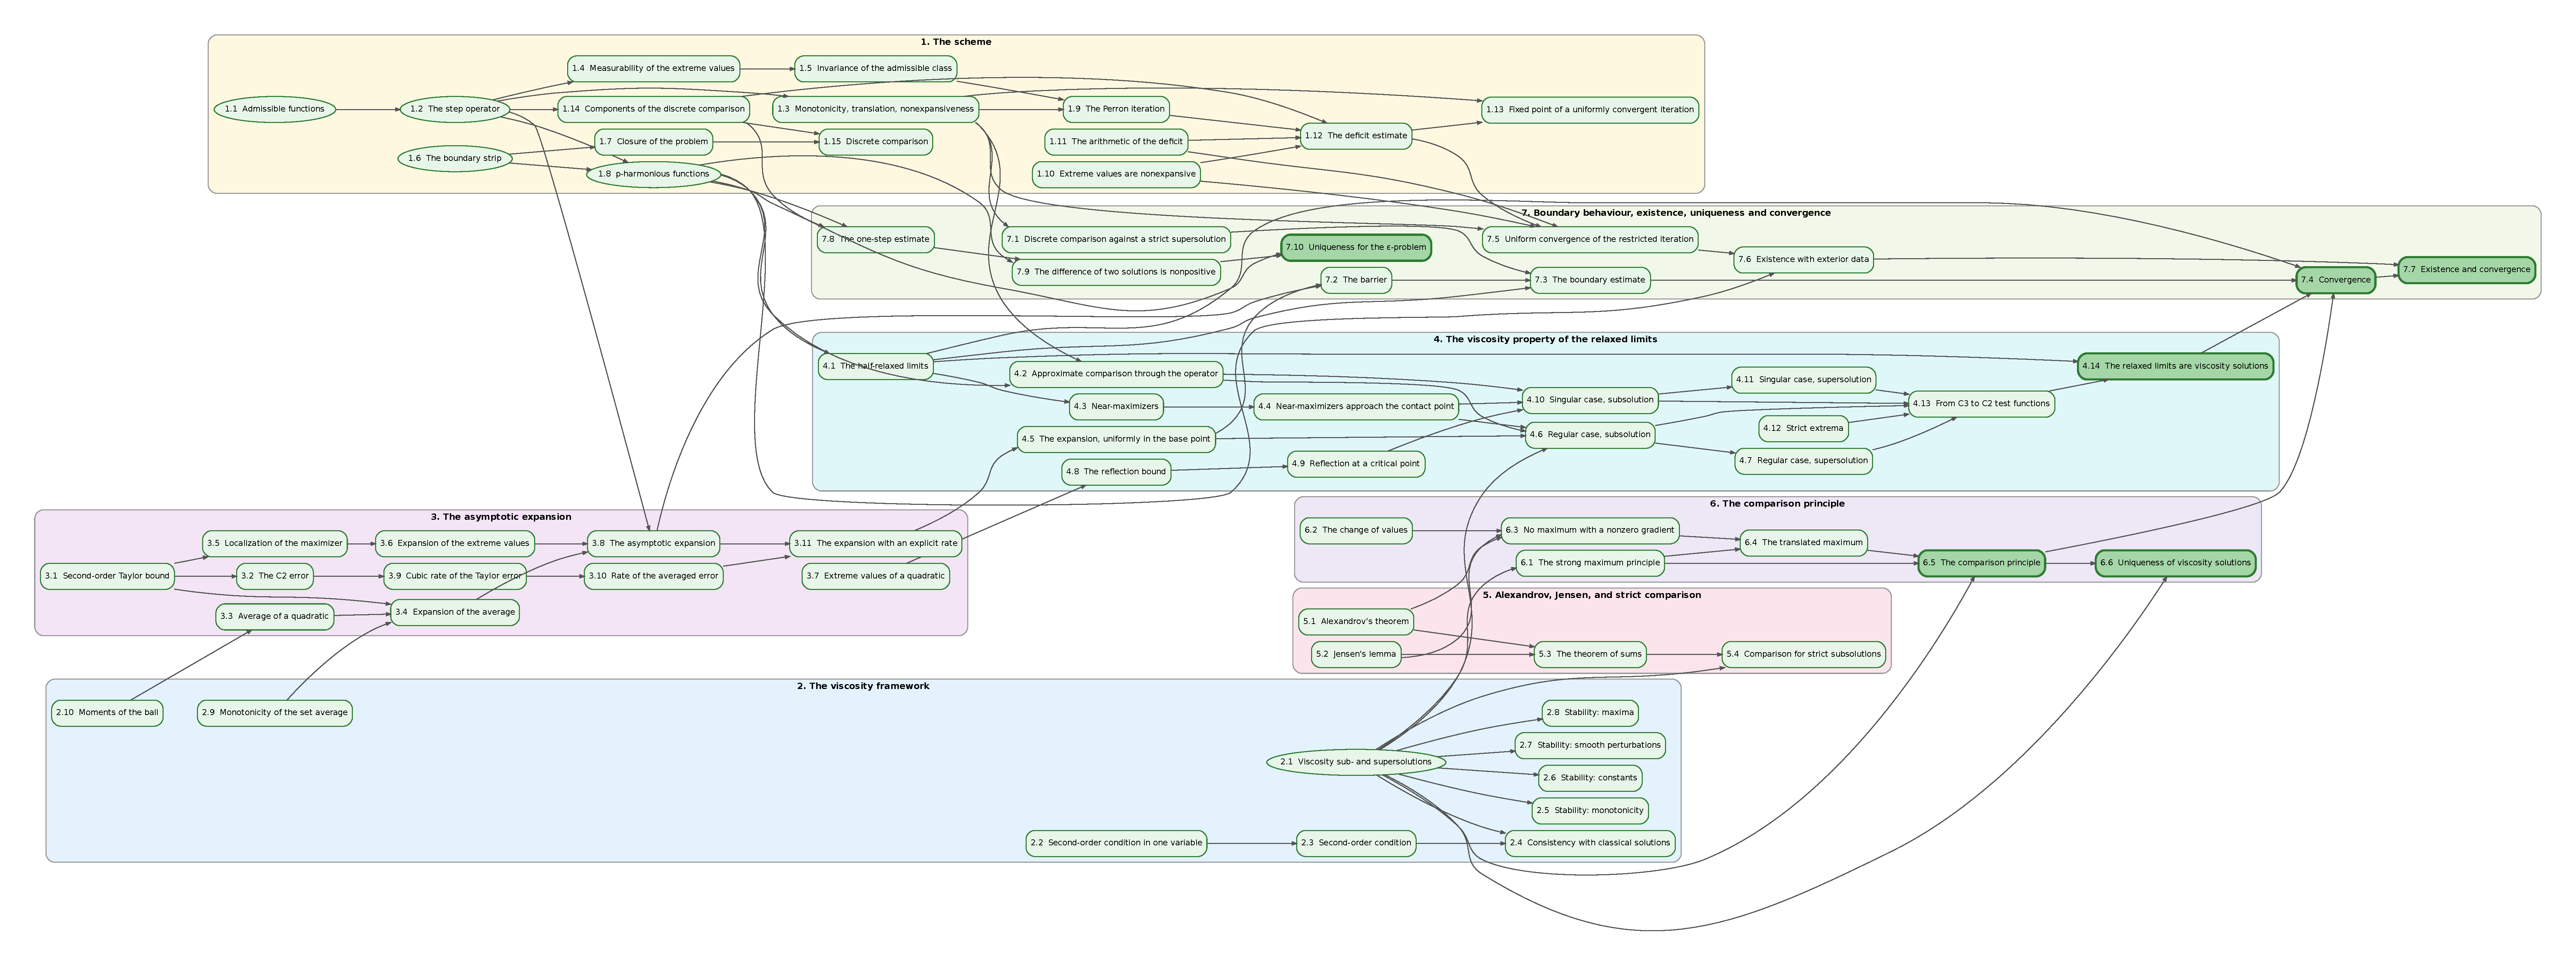
\includegraphics[width=\linewidth,height=0.85\textheight,keepaspectratio]{graph.pdf}
\caption{The dependency graph, by chapter. Arrows point from a result to the
results that use it; the main theorem is at the far right. The figure is
vector graphics and can be enlarged on screen.}\label{fig:graph}
\end{figure}
\end{landscape}
\chapter{The scheme}

\begin{definition}[Admissible functions]\label{def:bddmeas}
\lean{PLaplacian.BddMeas}
\leanok
A function $v \colon \R^d \to \R$ is \emph{admissible} if it is Borel
measurable and bounded.
\end{definition}


\begin{definition}[The step operator]\label{def:op}
\lean{PLaplacian.tugOfWarOp}
\leanok
\uses{def:bddmeas}
For $\eps > 0$ and $v$ admissible,
\begin{equation}
  \Op v(x) = \frac{\alpha}{2}\Bigl(\sup_{B_\eps(x)} v + \inf_{B_\eps(x)} v\Bigr)
    + \beta \avgint_{B_\eps(x)} v .
\end{equation}
\end{definition}


\begin{theorem}[Monotonicity, translation, nonexpansiveness]\label{thm:one}
\lean{PLaplacian.tugOfWarOp_monotone,PLaplacian.tugOfWarOp_add_const,PLaplacian.tugOfWarOp_nonexpansive}
\leanok
\uses{def:op}
For $u,v$ admissible:
\emph{(i)} $u \le v$ implies $\Op u \le \Op v$
(\texttt{tugOfWarOp\_monotone});
\emph{(ii)} $\Op(v+K) = \Op v + K$ (\texttt{tugOfWarOp\_add\_const});
\emph{(iii)} $\abs{u-v} \le K$ implies $\abs{\Op u - \Op v} \le K$
(\texttt{tugOfWarOp\_nonexpansive}).
\end{theorem}

\begin{proof}
\leanok
Part (i) needs $2 \le p$ essentially: for $1<p<2$ the weight $\alpha$ is
negative and the $\sup+\inf$ term is anti-monotone. Part (ii) is where $\alpha+\beta=1$ enters;
(iii) follows from (i) and (ii).
\end{proof}


\begin{theorem}[Measurability of the extreme values]\label{thm:meas}
\lean{PLaplacian.measurable_sSup_ball,PLaplacian.measurable_sInf_ball}
\leanok
\uses{def:op}
For $\eps>0$ and bounded $v$, the maps $x \mapsto \sup_{B_\eps(x)} v$ and
$x \mapsto \inf_{B_\eps(x)} v$ are Borel measurable.
\end{theorem}

\begin{proof}
\leanok
The proof is the reason for open balls: for every $\lambda$,
\begin{equation}
  \Bigl\{x : \sup_{B_\eps(x)} v > \lambda\Bigr\}
  = \bigcup_{\{y : v(y) > \lambda\}} B_\eps(y),
\end{equation}
a union of open balls.
\end{proof}


\begin{theorem}[Invariance of the admissible class]\label{thm:invariance}
\lean{PLaplacian.BddMeas.tugOfWarOp}
\leanok
If $v$ is admissible then so is $\Op v$.
\end{theorem}

\begin{proof}
\leanok
\uses{thm:meas}
This makes the existence iteration meaningful, and it is \emph{false} for
closed balls. Measurability of the average term is separate from
Theorem~\ref{thm:meas}: it is proved by rewriting the integral over the moving
ball as an integral over a fixed ball of a translated integrand and appealing
to \texttt{StronglyMeasurable.integral\_prod\_right}. Preservation of the
bound is convexity.
\end{proof}


\begin{definition}[The boundary strip]\label{def:strip}
\lean{PLaplacian.bdryStrip,PLaplacian.closureEps}
\leanok
$\Gamma_\eps = \{x \notin \Omega : \operatorname{dist}(x,\Omega) \le \eps\}$
and $\Omega_\eps = \Omega \cup \Gamma_\eps$.
\end{definition}


\begin{lemma}[Closure of the problem]\label{lem:closed}
\lean{PLaplacian.closedBall_subset_union}
\leanok
\uses{def:strip}
For $x \in \Omega$, $\overline{B}_\eps(x) \subseteq \Omega_\eps$.
\end{lemma}

\begin{proof}
\leanok
See the companion for the argument.
\end{proof}


\begin{definition}[p-harmonious functions]\label{def:pharm}
\lean{PLaplacian.IsPHarmonious}
\leanok
\uses{def:op,def:strip}
Given bounded Borel $F$ on $\Gamma_\eps$, a function $u$ is
\emph{$p$-harmonious with data $F$} if it is admissible, $u = \Op u$ on
$\Omega$, and $u = F$ on $\Gamma_\eps$.
\end{definition}


\begin{theorem}[The Perron iteration]\label{thm:iteration}
\lean{PLaplacian.iter}
\leanok
From an admissible $u_0$ with $u_0 \le \Op u_0$, the sequence
$u_{j+1} = \Op u_j$ has every term admissible, increases, inherits the bound on
$u_0$, converges pointwise to $u = \sup_j u_j$, and $u$ is admissible.
\end{theorem}

\begin{proof}
\leanok
\uses{thm:one,thm:invariance}
See the companion for the argument.
\end{proof}


\begin{theorem}[Extreme values are nonexpansive]\label{thm:unifcont}
\lean{PLaplacian.abs_sSup_sub_sSup_le}
\leanok
If $\abs{u-v} \le K$ pointwise then each of the three terms of $\Op$ changes by
at most $K$.
\end{theorem}

\begin{proof}
\leanok
Pointwise convergence would not suffice: the extreme-value terms are suprema
over a ball, and a pointwise limit need not have the limit of the suprema as
its supremum.  remark that $\beta>0$ is needed both for uniform
convergence and for the limit to satisfy the equation;
Theorem~\ref{thm:unifcont} is where the second use appears.
\end{proof}


\begin{theorem}[The arithmetic of the deficit]\label{thm:unifarith}
\lean{PLaplacian.unif_arith,PLaplacian.le_zero_of_forall_lt}
\leanok
Let $\alpha \ge 0$ with $\alpha+\beta=1$. If
$M - 2\delta \le \alpha S + \beta A$ with $S \le M+\delta$ and
$\beta A \le \delta$, then $\beta M \le \delta(3+\alpha)$. If moreover
$\beta>0$ and this holds for every $\delta>0$, then $M \le 0$.
\end{theorem}

\begin{proof}
\leanok
See the companion for the argument.
\end{proof}


\begin{theorem}[The deficit estimate]\label{thm:unifconv}
\lean{PLaplacian.deficitLimit_eq_zero}
\leanok
Let $M = \lim_j \sup_{\Omega_\eps}(u - u_j)$. Given the convergence of the
integrals of the deficit over $\Omega_\eps$ and the selections of the indices
and the point described below, $M \le 0$.
\end{theorem}

\begin{proof}
\leanok
\uses{thm:iteration,thm:unifcont,thm:unifarith,thm:comparison}
This is the substantive step. Following  one supposes
$M>0$, fixes $\delta>0$, chooses an index $k$, a point $x_0$ nearly attaining
the deficit supremum at stage $k+1$, and a late index $\ell$, and chains
\[
  M - 2\delta \le \alpha \sup_{B_\eps(x_0)}(u - u_k)
    + \beta \avgint_{B_\eps(x_0)}(u - u_k)
  \le \alpha(M+\delta) + \delta,
\]
whence $\beta M \le \delta(3+\alpha)$ and, $\beta$ being positive, $M \le 0$.
Four of the findings recorded in the companion arose here.
\end{proof}


\begin{theorem}[Fixed point of a uniformly convergent iteration]\label{thm:existence}
\lean{PLaplacian.exists_fixedPoint}
\leanok
Under the hypotheses of Theorem~\ref{thm:iteration} together with uniform
convergence, the limit is admissible and satisfies $\Op u = u$.
\end{theorem}

\begin{proof}
\leanok
\uses{thm:unifconv,thm:one}
The fixed-point property follows by passing the operator through the limit:
$\Op u$ is within $\eta$ of $\Op u_N$ by nonexpansiveness, and
$\Op u_N = u_{N+1}$ is within $\eta$ of $u$ by uniform convergence.
\end{proof}


\begin{theorem}[Components of the discrete comparison]\label{thm:comparison}
\lean{PLaplacian.key_estimate,PLaplacian.ae_eq_of_setAverage_eq_max,PLaplacian.measure_diff_max_set,PLaplacian.inner_advance,PLaplacian.max_set_unbounded,PLaplacian.not_bounded_max_set}
\leanok
\uses{def:op}
For $u,v$ admissible:
\emph{(i)} \emph{(\texttt{key\_estimate})}
$\Op v(x) - \Op u(x) \le \alpha \sup_{B_\eps(x)}(v-u)
  + \beta \avgint_{B_\eps(x)}(v-u)$;
\emph{(ii)} \emph{(\texttt{ae\_eq\_of\_setAverage\_eq\_max})} a function
bounded by $M$ whose average equals $M$ equals $M$ almost everywhere;
\emph{(iii)} \emph{(\texttt{measure\_diff\_max\_set})} at an attained maximum
the maximum set has full measure in the ball;
\emph{(iv)} \emph{(\texttt{inner\_advance})} displacement by
$\tfrac{\eps}{2}e$ advances $\langle e,\cdot\rangle$ by at least
$\tfrac{\eps}{4}$;
\emph{(v)} \emph{(\texttt{max\_set\_unbounded})} the maximum set is unbounded
in every direction;
\emph{(vi)} \emph{(\texttt{not\_bounded\_max\_set})} hence it cannot lie in a
bounded set.
\end{theorem}

\begin{proof}
\leanok
See the companion for the argument.
\end{proof}


\begin{theorem}[Discrete comparison]\label{thm:comparisonfinal}
\lean{PLaplacian.comparison_of_attained}
\leanok
Let $u,v$ be $p$-harmonious on a bounded $\Omega$, and $M$ such that
$v-u \le M$ everywhere and $v-u=M$ only inside $\Omega$. Then $v-u$ does not
attain $M$.
\end{theorem}

\begin{proof}
\leanok
\uses{thm:comparison,lem:closed}
At an attained maximum both functions equal their operator values, so the
difference is preserved by $\Op$, which supplies the fixed-point hypothesis of
(vi).
\end{proof}


\chapter{The viscosity framework}

\begin{definition}[Viscosity sub- and supersolutions]\label{def:sub}
\lean{PLaplacian.IsViscositySubsolution}
\leanok
An upper semicontinuous $u$ on $\Omega$ is a \emph{viscosity subsolution} of
$-\pnlap u = f$ if for every $\varphi \in C^2$ and every $x_0 \in \Omega$ at
which $u - \varphi$ has a local maximum,
\[
  F(\nabla\varphi(x_0), D^2\varphi(x_0)) \le f(x_0)
  \quad\text{when } \nabla\varphi(x_0) \ne 0,
\]
and $F_*(D^2\varphi(x_0)) \le f(x_0)$ when $\nabla\varphi(x_0) = 0$.
Supersolutions (\texttt{IsViscositySupersolution}) reverse the inequalities,
test from below, and use $F^*$; a solution is both.
\end{definition}


\begin{theorem}[Second-order condition in one variable]\label{thm:so1}
\lean{PLaplacian.IsLocalMax.deriv_deriv_nonpos}
\leanok
At an interior local maximum of a $C^2$ function of one real variable, the
second derivative is nonpositive; dually at a minimum.
\end{theorem}

\begin{proof}
\leanok
Mathlib's \texttt{Analysis.Calculus.LocalExtr.Basic} has Fermat's theorem and
its tangent-cone refinements, but nothing of second order. Our proof avoids Taylor's theorem: if the second
derivative were positive, continuity would keep it positive on an interval, so
the first derivative would be strictly increasing there; being zero at the
point by Fermat, it would then be positive to the right, making the function
strictly increasing and contradicting the maximum. Each step is an application
of \texttt{strictMonoOn\_of\_deriv\_pos}.
\end{proof}


\begin{theorem}[Second-order condition]\label{thm:somulti}
\lean{PLaplacian.hess_nonpos_of_isLocalMax}
\leanok
At a local maximum of a $C^2$ function on $\R^d$ the Hessian is nonpositive as
a quadratic form.
\end{theorem}

\begin{proof}
\leanok
\uses{thm:so1}
The proof restricts to a line through the point. Three steps: the restriction
attains a local maximum at the origin
(\texttt{IsLocalMax.along\_line}); its first derivative is the Fréchet
derivative applied to the direction (\texttt{hasDerivAt\_first}); and its
second derivative is the Hessian at the direction twice
(\texttt{hasDerivAt\_second}). The third is the
\texttt{iteratedDeriv}-against-\texttt{iteratedFDeriv} glue identified in our
initial gap audit as the likely friction point of the whole development. It is
resolved by \texttt{ContDiff.fderiv\_right}, which gives that the derivative
map of a $C^2$ function is itself $C^1$, followed by two chain rules and the
observation that evaluation at a fixed vector is continuous linear.
\end{proof}


\begin{theorem}[Consistency with classical solutions]\label{thm:consistency}
\lean{PLaplacian.viscF_le_of_classical}
\leanok
\uses{def:sub}
Let $u, \varphi$ be $C^2$, let $u - \varphi$ have a local maximum at $x_0$ with
$\nabla\varphi(x_0) \ne 0$, and suppose $u$ satisfies the operator inequality
at $x_0$. Then so does $\varphi$.
\end{theorem}

\begin{proof}
\leanok
\uses{thm:somulti}
Three inputs: the derivatives agree at the contact point, by Fermat
(\texttt{fderiv\_eq\_of\_isLocalMax}, and its gradient form via
\texttt{ext\_inner\_right}); the Hessians are ordered, by
Theorem~\ref{thm:somulti} applied to $u - \varphi$
(\texttt{hess\_le\_of\_isLocalMax}); and degenerate ellipticity transfers the
inequality.
\end{proof}


\begin{theorem}[Stability: monotonicity]\label{thm:stab-mono}
\lean{PLaplacian.IsViscositySubsolution.mono}
\leanok
\uses{def:sub}
A subsolution on $\Omega$ restricts to a subsolution on any subset, and dually.
\end{theorem}

\begin{proof}
\leanok
See the companion for the argument.
\end{proof}


\begin{theorem}[Stability: constants]\label{thm:stab-const}
\lean{PLaplacian.IsViscositySubsolution.add_const}
\leanok
\uses{def:sub}
If $u$ is a subsolution then so is $u + c$ for any constant $c$.
\end{theorem}

\begin{proof}
\leanok
The operator sees only the gradient and the Hessian, both unaffected. The proof
observes that testing $u+c$ against $\varphi$ is testing $u$ against
$\varphi - c$, and needs \texttt{gradient\_add\_const} and
\texttt{hess\_add\_const}, neither of which Mathlib has in gradient or Hessian
form.
\end{proof}


\begin{theorem}[Stability: smooth perturbations]\label{thm:stab-smooth}
\lean{PLaplacian.IsViscositySubsolution.add_smooth}
\leanok
\uses{def:sub}
If $u$ is a subsolution and $\psi$ is $C^2$, then at a contact point of
$u + \psi$ with a test function $\varphi$,
\[
  F\bigl(\nabla\varphi(x_0) - \nabla\psi(x_0),\,
    D^2\varphi(x_0) - D^2\psi(x_0)\bigr) \le f(x_0).
\]
\end{theorem}

\begin{proof}
\leanok
This cannot be converted into an inequality for $\varphi$ alone, because $F$ is
not additive in either argument --- the third appearance of that
non-additivity. The version stated is the honest
one, and also the usable one, since a convergence proof applies the subsolution
property to a perturbed test function and needs exactly this.
\end{proof}


\begin{theorem}[Stability: maxima]\label{thm:stab-max}
\lean{PLaplacian.IsViscositySubsolution.max,PLaplacian.IsViscositySubsolution.finsetSup'}
\leanok
\uses{def:sub}
The maximum of two subsolutions is a subsolution, and hence so is the maximum
over any nonempty finite family. Dually for minima of supersolutions.
\end{theorem}

\begin{proof}
\leanok
The argument is a case split on which function attains the maximum at the
contact point: if $u(x_0)$ attains it, then $u - \varphi$ has a local maximum
at $x_0$ too, since
$u(y) - \varphi(y) \le \max(u,v)(y) - \varphi(y) \le \max(u,v)(x_0) -
\varphi(x_0) = u(x_0) - \varphi(x_0)$. The finite case follows by induction.
The infinite case is a different theorem; see the companion.
\end{proof}


\begin{theorem}[Monotonicity of the set average]\label{thm:avgmono}
\lean{PLaplacian.setAverage_mono}
\leanok
For $\mu$ a measure, $s$ measurable, and $f \le g$ integrable on $s$:
$\avgint_s f \le \avgint_s g$.
\end{theorem}

\begin{proof}
\leanok
No hypothesis on $\mu(s)$ is needed: the unfolding
$\avgint_s f = \mu(s)^{-1}\!\int_s f$ is unconditional, and $\mu(s)^{-1}$ is
nonnegative even when $\mu(s) \in \{0,\infty\}$, where the junk-value
convention makes it $0$.
The lemma is absent from Mathlib at the revision this development pins, and is
a natural candidate for a pull request.
\end{proof}


\begin{theorem}[Moments of the ball]\label{thm:moments}
\lean{PLaplacian.integral_coord_ball_eq_zero,PLaplacian.integral_mul_coord_ball_eq_zero,PLaplacian.setAverage_sq_coord_unitBall}
\leanok
For $r>0$, $d \ge 1$ and $i \ne j$:
$\int_{B_r(0)} z_i = 0$, $\int_{B_r(0)} z_i z_j = 0$, and
$\avgint_{B_1(0)} z_i^2 = 1/(d+2)$.
\end{theorem}

\begin{proof}
\leanok
Three mechanisms. Odd moments follow from $z \mapsto -z$. Off-diagonal moments
need a reflection in a \emph{single} coordinate, since negating all of them
leaves $z_i z_j$ fixed; Mathlib has no such map, so we build it as a linear
isometry equivalence (\texttt{flipCoordEquiv}). Diagonal moments admit no
reflection argument: one sums over coordinates, uses
$\sum_i z_i^2 = \abs{z}^2$, and divides by $d$ using invariance under
coordinate permutations, which is free from
\texttt{LinearIsometryEquiv.piLpCongrLeft}. The radial reduction is
\texttt{integral\_fun\_norm\_addHaar}, whose presence in Mathlib was the most
consequential finding of our initial audit: it is the difference between a
routine development and a research problem.
\end{proof}


\chapter{The asymptotic expansion}

\begin{theorem}[Second-order Taylor bound]\label{thm:taylor}
\lean{PLaplacian.taylor_two_bounded}
\leanok
For $\varphi \in C^3$ and any $x, z$ there is a constant $C$, depending on $z$,
with
\[
  \Bigl\lvert \varphi(x+z) - \varphi(x) - D\varphi(x)z
    - \tfrac12 D^2\varphi(x)(z,z) \Bigr\rvert \le \frac{C}{6} .
\]
\end{theorem}

\begin{proof}
\leanok
See the companion for the argument.
\end{proof}


\begin{theorem}[The C2 error]\label{thm:ctwo}
\lean{PLaplacian.err2_le,PLaplacian.exists_taylorErr_le}
\leanok
For $\varphi \in C^2$, $x$ and $\eta > 0$ there is $\delta > 0$ with
\[
  \Bigl\lvert \varphi(x+w) - \varphi(x) - D\varphi(x)w
    - \tfrac12 D^2\varphi(x)(w,w) \Bigr\rvert \le \eta \norm{w}^2
  \qquad\text{for } \norm{w} < \delta .
\]
\end{theorem}

\begin{proof}
\leanok
\uses{thm:taylor}
No third derivative appears. The route is:
\end{proof}


\begin{theorem}[Average of a quadratic]\label{thm:quadavg}
\lean{PLaplacian.setAverage_quadratic}
\leanok
For a continuous bilinear form $X$ and $\eps > 0$,
\[
  \avgint_{B_\eps(0)} X(z,z)\,dz = \frac{\eps^2}{d+2}\,\Lambda(X) .
\]
\end{theorem}

\begin{proof}
\leanok
\uses{thm:moments}
This is the theorem the moment computations of Theorem~\ref{thm:moments} were
built for. Expanding $X(z,z)$ in coordinates, the off-diagonal terms vanish by
the mixed moments and the diagonal terms each contribute $\eps^2/(d+2)$, so
the surviving sum is the trace. The moments were stated for the unit ball and
had to be redone at radius $\eps$; the companion records why the
obvious route failed.
\end{proof}


\begin{theorem}[Expansion of the average]\label{thm:avgexp}
\lean{PLaplacian.setAverage_expansion}
\leanok
For $\varphi \in C^3$, $0 < \eps$ and $0 < d$,
\[
  \avgint_{B_\eps(x)} \varphi
    = \varphi(x) + \frac{\eps^2}{2(d+2)}\,\dlap\varphi(x)
      + \avgint_{B_\eps(0)} \mathrm{err} ,
\]
where $\mathrm{err}$ is the Taylor error of Theorem~\ref{thm:taylor}.
\end{theorem}

\begin{proof}
\leanok
\uses{thm:quadavg,thm:taylor,thm:avgmono}
The linear term vanishes by the odd moments; the quadratic term is
Theorem~\ref{thm:quadavg}. The error is left as an average rather than
estimated, so the statement is exact.
\end{proof}


\begin{theorem}[Localization of the maximizer]\label{thm:localize}
\lean{PLaplacian.localize_maximizer}
\leanok
Let $y$ maximize $\varphi$ on $\overline{B}_\eps(x)$, with
$\nabla\varphi(x) \ne 0$. If the Taylor errors at $y$ and at $x+\eps\nu$ differ
by at most $E$, then
\[
  \norm{y - x - \eps\nu}^2
  \le \frac{2\eps\bigl(\norm{D^2\varphi(x)}\eps^2 + E\bigr)}
           {\abs{\nabla\varphi(x)}} .
\]
\end{theorem}

\begin{proof}
\leanok
\uses{thm:taylor}
Our own analysis had identified this as the hardest single step in the
project. It reduces to a polarization identity. Since $y$ maximizes,
$\varphi(y) \ge \varphi(x+\eps\nu)$, and expanding both about $x$ makes the
linear functional nearly maximal on the ball; since that functional attains
its maximum only at $\eps\nu$, a deficit $c = \eps - \langle\nu, y-x\rangle$
bounds the squared distance, because
\[
  \norm{y - x - \eps\nu}^2
  = \norm{y-x}^2 - 2\eps\langle\nu, y-x\rangle + \eps^2
  \le 2\eps c
\]
using $\norm{y-x} \le \eps$. The Taylor comparison makes $c$ of order
$\eps^2$, so the maximizer lies within $O(\eps^{3/2})$ of the shifted point.
\end{proof}


\begin{theorem}[Expansion of the extreme values]\label{thm:extexp}
\lean{PLaplacian.sSup_lower_infLap,PLaplacian.sSup_upper_infLap}
\leanok
For $\varphi \in C^3$ with $\nabla\varphi(x) \ne 0$, the supremum over
$\overline{B}_\eps(x)$ is bounded below by
$\varphi(x) + \eps\abs{\nabla\varphi(x)}
  + \tfrac{\eps^2}{2}\inflap\varphi(x)$ plus the Taylor error at the shifted
point, and above by the same expression with the error at a maximizer plus
the quadratic comparison term.
\end{theorem}

\begin{proof}
\leanok
\uses{thm:localize}
The gap between the two is the difference of $D^2\varphi(x)$ at $y-x$ and at
$\eps\nu$, bounded by $\norm{D^2\varphi(x)}\,\norm{(y-x)-\eps\nu}\,
(\norm{y-x}+\eps)$ through the bilinear identity
$X(u,u) - X(v,v) = X(u-v,u) + X(v,u-v)$; with
Theorem~\ref{thm:localize} that is $O(\eps^{5/2})$.
\end{proof}


\begin{theorem}[Extreme values of a quadratic]\label{thm:singexp}
\lean{PLaplacian.quad_le_lamMax_ball}
\leanok
Where $\nabla\varphi(x) = 0$ the linear term is absent, and for
$\norm{z} \le \eps$, $z \ne 0$ and $\lambda_{\max}(X) \ge 0$,
\[
  X(z,z) \le \eps^2\,\lambda_{\max}(X) .
\]
\end{theorem}

\begin{proof}
\leanok
So at a singular point the expansion produces $\lambda_{\max}$ for the
supremum and $\lambda_{\min}$ for the infimum --- exactly the closed-form
envelopes of the viscosity predicates. The envelopes are therefore not a
convention but what the asymptotics give, which closes the circle between
Layers 2 and 3.
\end{proof}


\begin{theorem}[The asymptotic expansion]\label{thm:opexp}
\lean{PLaplacian.tugOfWarOp_expansion_final}
\leanok
\uses{def:op}
For $\varphi \in C^3$ with $\nabla\varphi(x) \ne 0$, $\eps > 0$, $0 < d$ and
$0 < p + d$, there is $E$ with
\[
  \Op\varphi(x) = \varphi(x)
    + \frac{\eps^2}{2(p+d)}\,\pnlap\varphi(x) + E .
\]
\end{theorem}

\begin{proof}
\leanok
\uses{thm:avgexp,thm:extexp}
Assembling: the extreme values of the operator are over \emph{open} balls and
the expansion was proved over closed ones, so
\texttt{sSup\_ball\_eq\_closedBall} is needed --- the one place in the
development where the choice of open balls must be paid for rather than
merely respected. Then the two halves are substituted and the weights
combined, with
\[
  \alpha \cdot \tfrac{\eps^2}{2} I
    + \beta \cdot \tfrac{\eps^2}{2(d+2)} L
  = \frac{\eps^2}{2(p+d)}\bigl[(p-2) I + L\bigr] ,
\]
the factor $d+2$ from the moments cancelling against $\beta$'s numerator.
\end{proof}


\begin{theorem}[Cubic rate of the Taylor error]\label{thm:cubicrate}
\lean{PLaplacian.taylorErr_le_cubic}
\leanok
For $\varphi \in C^3$, $x$ and $\eps$ there is $K$, independent of the
increment, with
\[
  \abs{\mathrm{err}(z)} \le K \norm{z}^3
  \qquad\text{for all } \norm{z} \le \eps .
\]
\end{theorem}

\begin{proof}
\leanok
\uses{thm:ctwo}
The cubic dependence is recovered by bounding the \emph{composition} rather
than identifying the third derivative pointwise. The third derivative of
$t \mapsto \varphi(x+tz)$ contains three factors of $z$, and
\texttt{norm\_iteratedFDeriv\_comp\_le} exposes them: with the line map's
derivatives bounded by $\norm{z}^i$ --- order one is exactly $\norm{z}$, and
all higher orders vanish, the map being affine --- the composition bound gives
$3!\,C\,\norm{z}^3$.
\end{proof}


\begin{theorem}[Rate of the averaged error]\label{thm:avgrate}
\lean{PLaplacian.setAverage_taylorErr_le}
\leanok
The average of the error over the ball satisfies
$\avgint_{B_\eps(0)} \mathrm{err} \le K\eps^3$.
\end{theorem}

\begin{proof}
\leanok
\uses{thm:cubicrate}
An average of a function bounded above by a constant is bounded by that
constant, which is \texttt{setAverage\_mono} against the constant function
--- the lemma of Theorem~\ref{thm:avgmono}, absent from Mathlib, used here for
the purpose it was proved for.
\end{proof}


\begin{theorem}[The expansion with an explicit rate]\label{thm:opbounded}
\lean{PLaplacian.tugOfWarOp_expansion_bounded}
\leanok
For $2 \le p$, if the two halves have errors bounded by $B_1$ and $B_2$, then
\[
  \Op\varphi(x) = \varphi(x)
    + \frac{\eps^2}{2(p+d)}\,\pnlap\varphi(x) + E ,
  \qquad \abs{E} \le B_1 + B_2 .
\]
\end{theorem}

\begin{proof}
\leanok
\uses{thm:opexp,thm:avgrate}
The weights satisfy $\abs{\alpha}, \abs{\beta} \le 1$ for $2 \le p$, so they do
not amplify: a rate for each half gives a rate for the total. Instantiating
with Theorem~\ref{thm:avgrate} and the localization estimate,
$\abs{E} = O(\eps^{5/2}) = o(\eps^2)$.
\end{proof}


\chapter{The viscosity property of the relaxed limits}

\begin{theorem}[The half-relaxed limits]\label{thm:relaxed}
\lean{PLaplacian.lbar_le_ubar,PLaplacian.upperSemicontinuous_ubar,PLaplacian.lowerSemicontinuous_lbar}
\leanok
\uses{def:pharm}
For a uniformly bounded family the two limits are finite and ordered, the
upper one is upper semicontinuous and the lower one lower semicontinuous.
\end{theorem}

\begin{proof}
\leanok
Finiteness requires the bound to be \emph{uniform} in $\eps$, and this is
where a fact recorded in the companion --- that the reals are not a complete
lattice, so an unbounded supremum is a junk value --- binds after being
recorded two layers earlier without consequence. The bound is available:
Theorem~\ref{thm:existence} bounds a solution by the bound on the initial
datum, with no dependence on $\eps$, so one datum serves the whole family.
\end{proof}


\begin{theorem}[Approximate comparison through the operator]\label{thm:approxcmp}
\lean{PLaplacian.dpp_comparison_approx}
\leanok
\uses{def:pharm}
Let $u$ be $p$-harmonious at $y \in \Omega$ for the parameter $\eps$, and let
$\varphi$ be bounded and measurable. If $u - \varphi \le c$ on $B_\eps(y)$ and
$u(y) - \varphi(y) \ge c - \kappa$, then
\[
  \varphi(y) \le \Op\varphi(y) + \kappa .
\]
\end{theorem}

\begin{proof}
\leanok
\uses{thm:one}
The proof uses three results of Layer~1 in one argument. Monotonicity pushes
$u \le \varphi + c$ through the operator, translation equivariance pulls the
constant out, and the dynamic programming principle replaces $\Op u(y)$ by
$u(y) \ge \varphi(y) + c - \kappa$.
\end{proof}


\begin{theorem}[Near-maximizers]\label{thm:nearsup}
\lean{PLaplacian.exists_near_sup_cube,PLaplacian.le_sup_on_ball}
\leanok
For each $\eps > 0$ there is $y_\eps \in \overline{B}_r(x_0)$ with
$S_\eps - \eps^3 < u_\eps(y_\eps) - \varphi(y_\eps)$, and
$u_\eps - \varphi \le S_\eps$ on $\overline{B}_r(x_0)$.
\end{theorem}

\begin{proof}
\leanok
\uses{thm:relaxed}
\emph{Convergence to the point of contact.} The standard argument extracts a
convergent subsequence of the $y_\eps$ and uses the strictness to identify its
limit. We do not extract a sequence.
\end{proof}


\begin{theorem}[Near-maximizers approach the contact point]\label{thm:nearfreq}
\lean{PLaplacian.nearmax_frequently_in_ball}
\leanok
For every $\rho > 0$, frequently as $\eps \to 0^+$, $y_\eps \in B_\rho(x_0)$.
\end{theorem}

\begin{proof}
\leanok
\uses{thm:nearsup}
The argument works on the annulus
$A = \overline{B}_r(x_0) \setminus B_\rho(x_0)$, in four steps.
\begin{enumerate}
  \item \emph{A gap on the annulus} (\texttt{annulus\_gap}).
        $\overline{u} - \varphi$ is upper semicontinuous and $A$ is compact, so
        the maximum over $A$ is attained
        (\texttt{UpperSemicontinuousOn.exists\_isMaxOn}); no point of $A$ is
        $x_0$, so by strictness it is $M - \eta$ for some $\eta > 0$.
  \item \emph{A uniform eventual bound} (\texttt{uniform\_bound\_annulus}).
        At each point of $A$ the family minus $\varphi$ is eventually below
        $M - \eta/2$ on a product neighbourhood; the neighbourhoods cover $A$,
        a finite subcover exists, and the intersection of the finitely many
        parameter sets is still a filter member. Mathlib has a lemma
        packaging this argument, \texttt{IsCompact.eventually\_forall\_of\_forall\_eventually},
        but it works with the two-sided neighbourhood of a pair, while the
        relaxed filter is one-sided in the parameter, so its hypothesis is
        stronger than the one available. The subcover is done by hand.
  \item \emph{The supremum is frequently large}
        (\texttt{frequently\_supBall\_large}). Near-contact gives, frequently
        on the product filter, a point of the ball with value above
        $M - \eta/4$, so $S_\eps > M - \eta/4$. That statement mentions the
        parameter alone, so it projects off the product filter
        (\texttt{frequently\_fst\_of\_prod}).
  \item \emph{Exclusion} (\texttt{nearmax\_in\_ball}). Frequently, then,
        $u_\eps(y_\eps) - \varphi(y_\eps) > S_\eps - \eps^3 > M - \eta/2$,
        which is incompatible with $y_\eps \in A$.
\end{enumerate}
Compactness is used once, on the annulus, to make a pointwise bound uniform;
everything else runs along the filter.
\end{proof}


\begin{theorem}[The expansion, uniformly in the base point]\label{thm:expunif}
\lean{PLaplacian.expansion_uniform,PLaplacian.eventually_bound_le}
\leanok
Let $\varphi \in C^3$ with $\nabla\varphi(x_0) \ne 0$. There are $\rho > 0$ and
constants $H, K, K_a \ge 0$ and $g > 0$ such that for every
$y \in B_\rho(x_0)$ and every $0 < \eps \le \rho$,
\[
  \Op\varphi(y) = \varphi(y) + \frac{\eps^2}{2(p+d)}\,\pnlap\varphi(y) + E,
  \qquad
  \abs{E} \le H\eps\sqrt{U} + (K + K_a)\,\eps^3,
  \quad
  U = \frac{2\eps(H\eps^2 + 2K\eps^3)}{g}.
\]
Moreover, for every $\eta > 0$, the bound is eventually at most $\eta\eps^2$.
\end{theorem}

\begin{proof}
\leanok
\uses{thm:opbounded}
The constants are chosen once, on a single ball, before the base point and the
parameter; the order of the quantifiers in the statement is its content. The
last assertion holds because the bound equals $\eps^2 q(\eps)$ with
$q(\eps) = H\sqrt{2\eps(H + 2K\eps)/g} + (K + K_a)\eps$, continuous and
vanishing at zero (\texttt{bound\_eq\_sq\_mul}, \texttt{tendsto\_errFactor}).
\end{proof}


\begin{theorem}[Regular case, subsolution]\label{thm:regsub}
\lean{PLaplacian.regular_subsol}
\leanok
\uses{def:sub}
Let $\overline{B}_r(x_0) \subseteq \Omega$, let $\varphi$ be bounded and of
class $C^3$, let $\overline{u} - \varphi$ have a strict maximum at $x_0$ on
$\overline{B}_r(x_0)$, and let $\nabla\varphi(x_0) \ne 0$. Then
$\pnlap\varphi(x_0) \ge 0$.
\end{theorem}

\begin{proof}
\leanok
\uses{thm:approxcmp,thm:nearfreq,thm:expunif}
See the companion for the argument.
\end{proof}


\begin{theorem}[Regular case, supersolution]\label{thm:regsup}
\lean{PLaplacian.regular_supsol}
\leanok
At a strict minimum of $\underline{u} - \varphi$, under the same hypotheses,
$\pnlap\varphi(x_0) \le 0$.
\end{theorem}

\begin{proof}
\leanok
\uses{thm:regsub}
This is obtained from Theorem~\ref{thm:regsub} by transport, with no part of
the argument repeated. The operator is odd,
$\Op(-v) = -\Op v$ (\texttt{tugOfWarOp\_neg}), the supremum and infimum
exchanging under negation; so the negated family is $p$-harmonious with negated
datum (\texttt{isPHarmonious\_neg}). A strict minimum of
$\underline{u} - \varphi$ is a strict maximum of
$\overline{(-u)} - (-\varphi)$, and $\pnlap(-\varphi) = -\pnlap\varphi$
(\texttt{normPLapOf\_neg}). Transport through negation was available for the
operator because the operator happens to be odd; it is not available for the
comparison of Theorem~\ref{thm:approxcmp}, which uses monotonicity in one
direction only.
\end{proof}


\begin{theorem}[The reflection bound]\label{thm:reflect}
\lean{PLaplacian.reflect_bound}
\leanok
If $\abs{E_y(z)} \le K\eps^3$ for $\abs{z} \le \eps$, there is $z$ with
$\abs{z} \le \eps$ and
\[
  \tfrac12\Bigl(\sup_{\overline{B}_\eps(y)}\varphi + \inf_{\overline{B}_\eps(y)}\varphi\Bigr)
  \le \varphi(y) + \tfrac12 D^2\varphi(y)(z,z) + K\eps^3 .
\]
\end{theorem}

\begin{proof}
\leanok
\uses{thm:singexp}
No gradient enters. Bounding
$D^2\varphi(y)(z,z) \le (\lambda_{\max}^+(X) + \eta)\,\eps^2$, with
$\lambda^+ = \max(\lambda, 0)$, uses the quadratic bound
$X(z,z) \le \lambda_{\max}(X)\abs{z}^2$ for \emph{every} $z$
(\texttt{quad\_le\_lamMax\_norm}) --- the layer-two version covers only
$\lambda_{\max} \ge 0$ and nonzero $z$, and the negative case is exactly where
the argument lives --- together with continuity of the Hessian in the operator
norm, uniformly in the direction (\texttt{hess\_quad\_cont}). That continuity
is unavailable for the curried Hessian; it is obtained by writing the
difference of the two quadratic forms as the \emph{flat} second derivative
applied to $(z,z)$ (\texttt{iteratedFDeriv\_two\_apply}) and bounding it by
that map's operator norm. Pushing through the comparison as in the regular case
gives, in the limit,
\[
  0 \le (p-2)\,\lambda_{\max}^+(X) + \Lambda(X).
\]
This involves $\lambda_{\max}^+$, not $\lambda_{\max}$, which is why the
stronger bound fails --- but it suffices.
\end{proof}


\begin{lemma}[Reflection at a critical point]\label{lem:reflectneg}
\lean{PLaplacian.reflect_neg_of_envelope_pos}
\leanok
If $F_*(X) > 0$ then $(p-2)\lambda_{\max}^+(X) + \Lambda(X) < 0$.
\end{lemma}

\begin{proof}
\leanok
\uses{thm:reflect}
See the companion for the argument.
\end{proof}


\begin{theorem}[Singular case, subsolution]\label{thm:singsub}
\lean{PLaplacian.singular_subsol}
\leanok
Let $\overline{B}_r(x_0) \subseteq \Omega$, let $\varphi$ be bounded and of
class $C^3$, and let $\overline{u} - \varphi$ have a strict maximum at $x_0$ on
$\overline{B}_r(x_0)$. Then $F_*(D^2\varphi(x_0)) \le 0$.
\end{theorem}

\begin{proof}
\leanok
\uses{lem:reflectneg,thm:approxcmp,thm:nearfreq}
There is no hypothesis on the gradient. The inequality holds at every strict
maximum, singular or not; at a regular point it is weaker than
Theorem~\ref{thm:regsub}, since $\mathcal{I}_q(X) \le \lambda_{\max}(X)$.
\end{proof}


\begin{theorem}[Singular case, supersolution]\label{thm:singsup}
\lean{PLaplacian.singular_supsol}
\leanok
At a strict minimum of $\underline{u} - \varphi$,
$F^*(D^2\varphi(x_0)) \ge 0$.
\end{theorem}

\begin{proof}
\leanok
\uses{thm:singsub}
By transport, using $\lambda_{\max}(-X) = -\lambda_{\min}(X)$
(\texttt{lamMax\_neg}). The proof of Theorem~\ref{thm:singsub} is the longest
single declaration in the development, and its first version timed out.
\end{proof}


\begin{theorem}[Strict extrema]\label{thm:regularize}
\lean{PLaplacian.regularize}
\leanok
Let $\varphi \in C^3$ and let $V - \varphi$ have a local maximum at $x_0$. For
every $R > 0$ there are a bounded $\psi \in C^3$ and $0 < r \le R$ such that
$V - \psi$ has a strict maximum at $x_0$ on $\overline{B}_r(x_0)$,
$\nabla\psi(x_0) = \nabla\varphi(x_0)$ and
$D^2\psi(x_0) = D^2\varphi(x_0)$.
\end{theorem}

\begin{proof}
\leanok
The statement is for a generic $V$, so that it serves the supersolution through
$V = \overline{(-u)}$. With it, the four core theorems extend to $C^3$ test
functions at arbitrary local extrema; this is recorded as the predicates
\texttt{IsViscositySubsolution3} and \texttt{IsViscositySupersolution3},
identical to the layer-two ones except for the class of test function
(\texttt{ubar\_isViscositySubsolution3},
\texttt{lbar\_isViscositySupersolution3}).
\end{proof}


\begin{theorem}[From C3 to C2 test functions]\label{thm:c2reduce}
\lean{PLaplacian.visc2_reg_sub,PLaplacian.visc2_sing_sub,PLaplacian.visc2_reg_super,PLaplacian.visc2_sing_super}
\leanok
The four fields of the layer-two predicates hold for $\overline{u}$ and
$\underline{u}$ with $C^2$ test functions at local extrema.
\end{theorem}

\begin{proof}
\leanok
\uses{thm:regsub,thm:regsup,thm:singsub,thm:singsup,thm:regularize}
See the companion for the argument.
\end{proof}


\begin{theorem}[The relaxed limits are viscosity solutions]\label{thm:main4}
\lean{PLaplacian.ubar_isViscositySubsolution,PLaplacian.lbar_isViscositySupersolution}
\leanok
Let $2 \le p < \infty$, $d \ge 1$, and let $\Omega \subseteq \R^d$ be open.
Let $F$ be a boundary datum and $(u_\eps)$ a family of functions with
$\abs{u_\eps} \le C$ uniformly, each $u_\eps$ being $p$-harmonious in $\Omega$
with datum $F$. Then $\overline{u}$ is a viscosity subsolution and
$\underline{u}$ a viscosity supersolution of $-\pnlap u = 0$ in $\Omega$, in
the sense of Definition~\ref{def:sub}.
\end{theorem}

\begin{proof}
\leanok
\uses{thm:c2reduce,thm:relaxed}
The theorem is stated against the layer-two predicates exactly as they were
defined: $C^2$ test functions, arbitrary local extrema, and both the regular
and the singular fields. No restricted class of test function remains in the
statement. Neither boundedness of $\Omega$ nor any regularity of $F$ is used.
\end{proof}


\chapter{Alexandrov, Jensen, and strict comparison}

\begin{theorem}[Alexandrov's theorem]\label{thm:alexandrov}
\lean{PLaplacian.alexandrov}
\leanok
A convex function $f\colon \R^d \to \R$ is twice differentiable in the sense of
Peano at almost every point: for almost every $x$ there are $q \in \R^d$ and a
bilinear form $X$ with
\[
  f(x + h) = f(x) + \langle q, h\rangle + \tfrac12 X(h, h) + o(|h|^2).
\]
\end{theorem}

\begin{proof}
\leanok
\emph{The proximal map.} For each $y$ the function
$x \mapsto f(x) + \tfrac12 |x - y|^2$ has a unique minimizer $J(y)$; the
difference $y - J(y)$ is a subgradient at $J(y)$; conversely $J(x + p) = x$
whenever $p$ is a subgradient at $x$; and $J$ is one-Lipschitz
(\texttt{prox\_exists}, \texttt{prox\_unique}, \texttt{prox\_subgrad},
\texttt{prox\_of\_subgrad}, \texttt{prox\_lipschitz}).
\end{proof}


\begin{theorem}[Jensen's lemma]\label{thm:jensen}
\lean{PLaplacian.jensen_positive_measure,PLaplacian.jensen}
\leanok
Let $W\colon \R^n \to \R$ be such that $W + \tfrac C2 |\cdot|^2$ is convex, and
suppose $W(y) + 2\delta r < W(x_s)$ whenever $|y - x_0| = r$, for some
$x_s \in \overline B(x_0, r)$. Then the set of points of $B(x_0, r)$ at which
some tilt $W + \langle p, \cdot\rangle$ with $|p| \le \delta$ attains its
maximum over $\overline B(x_0, r)$ has positive measure.
\end{theorem}

\begin{proof}
\leanok
Let $Q(x)$ be a subgradient of $W + \tfrac C2|\cdot|^2$ at $x$ and
$g(x) = Cx - Q(x)$. At a point of the set the tilt is forced, $p = g(x)$; every
tilt of norm at most $\delta$ is attained, the maximum being kept off the sphere
by the hypothesis, so $g$ maps the set onto a ball; and $g$ is Lipschitz, with
constant $3C$, on the parts of the set away from the sphere, because there $W$
is squeezed between its semiconvex lower bound and the upper bound that the
maximum provides. Were the set null, its image under $g$ would be null, being a
countable union of Lipschitz images of null sets; but the image contains a
ball.
\end{proof}


\begin{theorem}[The theorem of sums]\label{thm:sums}
\lean{PLaplacian.theoremOfSums_of_regular,PLaplacian.theoremOfSumsRegular_of}
\leanok
The theorem of sums in the form above holds on the diagonal outright, and off
the diagonal by Alexandrov's theorem and Jensen's lemma
(Theorems~\ref{thm:alexandrov} and~\ref{thm:jensen}), both of which are proved.
\end{theorem}

\begin{proof}
\leanok
\uses{thm:alexandrov,thm:jensen}
On the diagonal the zero forms are genuine jets. Off it the proof follows ,
with one simplification. After translating, absorbing the penalty gradient, and
subtracting $K|\xi|^4$, which makes the maximum strict, global, and the functions
bounded above for $K$ large (\texttt{exists\_K\_strict}), the penalty is
bounded by its exact second-order expansion (\texttt{penalty\_expand}), and
Young's inequality decouples it so that sup- and inf-convolutions of the two
functions, with parameter $\lambda = 8M + 1$, inherit the strict maximum
(\texttt{dblW0\_conv\_strict}). Jensen's lemma gives maxima of small linear
perturbations on a set of positive measure, Alexandrov's theorem makes both
convolutions twice differentiable almost everywhere, and at a common point the
second-order condition along the diagonal direction gives $X \le Y$ directly
(\texttt{core\_diag}). The magic property of
sup-convolutions (Crandall--Ishii--Lions, Lemma~A.5) carries the jets back to the
maximizers, which converge because the gradients do
(\texttt{superJet\_of\_supConv}, \texttt{supConv\_grad}); symmetrizing and
extracting in coordinates gives limit forms (\texttt{exists\_subseq\_form});
and the quartic, translation and gradient are added back
(\texttt{superJet\_u\_of\_uTilde}).
\end{proof}


\begin{theorem}[Comparison for strict subsolutions]\label{thm:strictcomp}
\lean{PLaplacian.comparison_strict_of_AJ,PLaplacian.comparison_strict_full}
\leanok
\uses{def:sub}
Assume Alexandrov's theorem and Jensen's lemma, in the forms
\texttt{AlexandrovThm} and \texttt{JensenLemma} below. Let
$\Omega \subseteq \R^d$ be bounded and open, $2 \le p$, and $c > 0$. Let $U$ be
bounded above and upper semicontinuous, and a viscosity subsolution of
$-\pnlap u = -c$ in $\Omega$; let $V$ be bounded below and lower semicontinuous,
and a viscosity supersolution of $-\pnlap u = 0$ in $\Omega$. If $U \le V$ on
$\partial\Omega$, then $U \le V$ in $\Omega$.
\end{theorem}

\begin{proof}
\leanok
\uses{thm:sums}
Alexandrov's theorem and Jensen's lemma are classical results of real analysis,
not of the theory of viscosity solutions. They entered first as hypotheses,
stated as propositions; both are now proved
(Theorems~\ref{thm:alexandrov} and~\ref{thm:jensen}), so the theorem holds
outright (\texttt{comparison\_strict\_full}). The proof was organized
so that each deep result was stated first and its consumer proved from it,
which fixed every interface before the analysis it rests on.
\end{proof}


\chapter{The comparison principle}

\begin{theorem}[The strong maximum principle]\label{thm:smp}
\lean{PLaplacian.smp_ball_jet,PLaplacian.smp_ball,PLaplacian.smp_ball_min}
\leanok
\uses{def:sub}
Let $u$ be upper semicontinuous on $\Omega$, and suppose that every superjet
$(q, X)$ of $u$ at a point of $\Omega$ with $q \ne 0$ satisfies
$F(q, X) \le 0$. If $u \le u(x)$ on $B(x, R) \subseteq \Omega$, then
$u \equiv u(x)$ on $B(x, R/3)$. In particular this holds for viscosity
subsolutions of $-\pnlap u = 0$; and supersolutions satisfy the corresponding
minimum principle, their negations being subsolutions
(\texttt{IsViscositySupersolution.neg}).
\end{theorem}

\begin{proof}
\leanok
Suppose $u(y_0) < m = u(x)$ near $x$, let $r$ be the distance from $y_0$ to the
closed contact set $\{u = m\}$, and $z$ a nearest contact point. On a thin
annulus about $y_0$ of outer radius $r$ the barrier
$\varphi = (|\cdot - y_0|^2 - B)^2$, with $B$ slightly larger than $r^2$, has
nonzero gradient, and a maximizer of $u + \eps\varphi$ over the annulus is a
genuine local maximum. There the exact expansion of $\varphi$ turns the
maximum into a superjet of $u$ (\texttt{superJet\_barrier}), at which
\[
  F = \eps\bigl[\,8(p - 1)s - 4(B - s)(d + p - 2)\,\bigr] \ge \eps(p-1)r^2 > 0,
  \qquad s = |w - y_0|^2,
\]
(\texttt{viscF\_barrierJet}), contradicting the hypothesis. The barrier is never
differentiated, only the regular case of the
predicates is used, and stating the hypothesis for jets lets the principle
apply to sup-convolutions directly.
\end{proof}


\begin{theorem}[The change of values]\label{thm:cv}
\lean{PLaplacian.peanoAt_cv,PLaplacian.normPLapOf_cv_strict,PLaplacian.semiconcave_psi}
\leanok
Let $\psi(s) = s - \eta s^2$ with $\eta > 0$. If $V$ has the Peano expansion
$(q, X)$ at $x$, then $\psi \circ V$ has the expansion
$(c q,\ cX - 2\eta\, q \otimes q)$, with $c = \psi'(V(x)) = 1 - 2\eta V(x)$; and
if $\pnlap(q, X) \le 0$, $q \ne 0$ and $c > 0$, then
\[
  \pnlap\bigl(c q,\ cX - 2\eta\, q\otimes q\bigr) \le -2\eta(p - 1)\,|q|^2 .
\]
If $V$ is semiconcave and $0 \le \psi'(V) \le C_c$ everywhere, then
$\psi \circ V$ is semiconcave.
\end{theorem}

\begin{proof}
\leanok
The strictness gained is proportional to $|q|^2$ and vanishes at critical points,
exactly as anticipated; the next two steps deal
with them. The composition is used only at points where $V$ is twice
differentiable, so no viscosity chain rule is needed.
\end{proof}


\begin{theorem}[No maximum with a nonzero gradient]\label{thm:step2}
\lean{PLaplacian.step2}
\leanok
Let $U$ be semiconvex and $V$ and $W = \psi \circ V$ semiconcave. Suppose $U$
satisfies the jet subsolution inequality and $V$ the jet supersolution
inequality on an open set $O \supseteq B(x, \rho)$, with
$0 < \psi'(V) \le C_c$ there. If $x$ is a maximum of $U - W$ on $B(x, \rho)$,
then every lower support $q$ of $U$ at $x$ vanishes.
\end{theorem}

\begin{proof}
\leanok
\uses{thm:cv,thm:alexandrov,thm:jensen}
Two quantitative ingredients replace the sequences of the textbook argument. First, a gradient estimate
(\texttt{grad\_est}): a lower support $a$ of $U$ at $y$ satisfies
$|a - q| \le (\lambda + 2\mu)\,|y - x|$, by testing in the direction of $a - q$
against the upper support that the maximum provides. Second, a single point:
suppose $q \ne 0$, and apply Jensen's lemma to
$U - W - \delta|\cdot - x|^2$, which is globally semiconvex as
$U - W - |\cdot - x|^4$ is not; the positive-measure set it yields meets the
sets on which Alexandrov's theorem makes $U$ and $-V$ twice differentiable, at a
point $y_0$ with tilt $\pi$. Reading off the conditions at the maximum there
(\texttt{max\_peano}) gives
\[
  a - c\,b = 2\delta(y_0 - x) - \pi, \qquad
  A \le cB - 2\eta\, b \otimes b + 2\delta I,
\]
and the operator estimates chain to
$0 \le -\kappa + \kappa/3 + \kappa/3$, with
$\kappa = 2\eta(p - 1)\bigl(|q|/(2C_c)\bigr)^2$ (\texttt{step2\_chain}).
\end{proof}


\begin{theorem}[The translated maximum]\label{thm:step3}
\lean{PLaplacian.step3}
\leanok
Under the hypotheses of Theorem~\ref{thm:step2}, let $G$ be bounded, open and
connected, with $B(x, R_0) \subseteq O$ for $x \in \overline G$. Then $U - W$
cannot be strictly larger at a point of $G$ than everywhere on $\partial G$.
\end{theorem}

\begin{proof}
\leanok
\uses{thm:step2,thm:smp}
Let $M(h) = \max_{\overline G}\bigl(U(\cdot + h) - W\bigr)$. For small $h$ the
maximizers are interior, by uniform continuity and the gap; at each,
Theorem~\ref{thm:step2} applies to the translate, so its lower support is zero
and
\[
  M(h + k) \ge M(h) - \tfrac\lambda2 |k|^2 .
\]
Splitting a segment into $N$ equal steps loses at most $\lambda|k|^2/(2N)$, so
$M$ is constant near $0$ (\texttt{const\_of\_quad\_lower}); no Lipschitz bound
or Rademacher's theorem is needed. On the contact set
$K = \{x \in G : U - W = M(0)\}$, $U$ has a local maximum, $W$ a local minimum
directly, and $V$ a local minimum because $\psi$ is increasing where $\psi' > 0$.
The two strong principles make $U$ and $V$ constant near each point of $K$, so
$K$ is open; it is relatively closed and nonempty, so connectedness gives
$K = G$, and continuity carries $U - W = M(0)$ to a frontier point, contradicting
the gap.
\end{proof}


\begin{theorem}[The comparison principle]\label{thm:viscomp}
\lean{PLaplacian.visc_comparison}
\leanok
\uses{def:sub}
Let $\Omega \subseteq \R^d$ be bounded and open, $d \ge 1$ and $2 \le p$. Let $U$
be bounded, upper semicontinuous, and a viscosity subsolution of
$-\pnlap u = 0$ in $\Omega$; let $V$ be bounded, lower semicontinuous, and a
viscosity supersolution. If $U \le V$ on $\partial\Omega$, then $U \le V$ in
$\Omega$.
\end{theorem}

\begin{proof}
\leanok
\uses{thm:step3,thm:smp}
The proof runs through a strong maximum principle, the change of values, and three steps:
no maximum of the regularized difference has a nonzero gradient; translated maxima are constant, and the contact set is
everything; and the regularization produces a set on which
the regularized difference exceeds its boundary values.
The theorem depends only on Lean's standard axioms.
\end{proof}

\begin{theorem}[Uniqueness of viscosity solutions]\label{thm:viscunique}
\lean{PLaplacian.visc_unique}
\leanok
\uses{def:sub}
Two bounded continuous viscosity solutions of $-\pnlap u = 0$ in a bounded open
set $\Omega$ that agree on $\partial\Omega$ agree in $\Omega$.
\end{theorem}

\begin{proof}
\leanok
\uses{thm:viscomp}
A viscosity solution is both a sub- and a supersolution, and a continuous
function is both upper and lower semicontinuous, so
Theorem~\ref{thm:viscomp} applies in each direction and gives
$u_1 \le u_2$ and $u_2 \le u_1$ in $\Omega$.
\end{proof}


\chapter{Boundary behaviour, existence, uniqueness and convergence}

\begin{theorem}[Discrete comparison against a strict supersolution]\label{thm:disccomp}
\lean{PLaplacian.disc_comparison}
\leanok
Let $u$ and $v$ be admissible, with $u = \Op u$ and $\Op v \le v - \kappa$ on a
set $D$ for some $\kappa > 0$, and $u \le v$ at the points outside $D$ within
$\eps$ of it. Then $u \le v$ on $D$.
\end{theorem}

\begin{proof}
\leanok
\uses{thm:one}
Each of the three terms of $\Op$ moves by at most $\sup_{B_\eps(x)}(u - v)$, so
$\Op u - \Op v$ does (\texttt{tugOfWarOp\_diff\_le}); hence
$u - v \le M - \kappa$ on $D$, with $M$ the supremum over the
$\eps$-neighbourhood, and $u - v \le 0$ outside $D$. Unlike
Theorem~\ref{thm:comparisonfinal}, which compares two solutions, this needs no
attained maximum.
\end{proof}


\begin{theorem}[The barrier]\label{thm:barrier}
\lean{PLaplacian.bpsi_op,PLaplacian.barrier_super}
\leanok
For a ball $B(z, \delta)$ let $s = |x - z|^2$, $t = s - \delta^2$ and
$\psi = t - M t^2$, with $M = (2(d + p - 2) + 1)/(8(p - 1)\delta^2)$. On the
shell $\delta^2 \le s \le \delta^2 + 1/(4M)$ the gradient of $\psi$ does not
vanish and $\pnlap \psi \le -1$; consequently, for $c \in \R$, $A > 0$ and
$\eps$ small,
\[
  \Op(c + A\psi) \le c + A\psi - \frac{A\eps^2}{4(p + d)}
\]
on the shell.
\end{theorem}

\begin{proof}
\leanok
\uses{thm:opexp,thm:expunif}
The barrier is a polynomial, hence globally smooth, which the expansion of
Layer~3 requires. Its expansion at a point is
exact algebra, and the value of $\pnlap$ at $(\nabla\psi, D^2\psi)$ is read off it
through the uniqueness of Peano expansions (\texttt{peano\_unique},
\texttt{normPLapOf\_of\_peano}), so no Hessian is computed. The expansion of Theorem~\ref{thm:expunif} becomes
uniform on the compact shell by a finite cover (\texttt{expansion\_compact}).
\end{proof}


\begin{theorem}[The boundary estimate]\label{thm:bdry}
\lean{PLaplacian.ubar_le_bdry}
\leanok
Let $|u_\eps| \le C$, with each $u_\eps$ $p$-harmonious in $\Omega$ with data
$F$ and equal to $F$ outside $\Omega$. Let $y_0$ have an exterior ball
$B(z_0, \delta_0)$ disjoint from $\Omega$, with $|y_0 - z_0| = \delta_0$, and let
$F$ be continuous at $y_0$. Then $\overline u(y_0) \le F(y_0)$.
\end{theorem}

\begin{proof}
\leanok
\uses{thm:barrier,thm:disccomp,thm:relaxed}
Halve the exterior ball, centring it at the midpoint $z$ of $y_0$ and $z_0$. By
Apollonius's identity,
$|x - z|^2 \ge \delta^2 + \tfrac12|x - y_0|^2$ for $x$ outside $B(z_0, \delta_0)$,
so the contact is unique and the region
$D = \Omega \cap \{|x - z|^2 < \delta^2 + \tau\}$ lies close to $y_0$. The
barrier $F(y_0) + \eta + A\psi$, clamped to make it admissible and unchanged on
the balls the operator reads (\texttt{tugOfWarOp\_congr\_ball}), dominates
$u_\eps$ on the $\eps$-neighbourhood of $D$ for $A$ large and $\eps$ small, and
Theorem~\ref{thm:disccomp} gives $u_\eps \le F(y_0) + 2\eta$ near $y_0$. The lower
estimate $F \le \underline u$ follows by applying the theorem to $-u_\eps$, which
is $p$-harmonious with data $-F$ because $\Op$ is odd. The hypothesis
$u_\eps = F$ outside $\Omega$ is essential.
\end{proof}


\begin{theorem}[Convergence]\label{thm:main}
\lean{PLaplacian.pharmonious_converge}
\leanok
Let $2 \le p$ and $d \ge 1$, let $\Omega \subseteq \R^d$ be bounded and open
with an exterior sphere at every boundary point, and let $F$ be continuous. Let
$(u_\eps)_{\eps > 0}$ be uniformly bounded, each $u_\eps$ $p$-harmonious in
$\Omega$ with data $F$ and equal to $F$ outside $\Omega$. Then
$\overline u = \underline u$ on $\overline\Omega$, $\overline u = F$ on
$\partial\Omega$, and $u_\eps \to \overline u$ uniformly on $\overline\Omega$.
\end{theorem}

\begin{proof}
\leanok
\uses{thm:main4,thm:bdry,thm:viscomp,thm:relaxed}
By Theorem~\ref{thm:main4}, $\overline u$ is a subsolution and $\underline u$ a
supersolution; by Theorem~\ref{thm:bdry} and its negation,
$\overline u \le F \le \underline u$ on $\partial\Omega$; so
Theorem~\ref{thm:viscomp} gives $\overline u \le \underline u$ in $\Omega$, and
with Theorem~\ref{thm:relaxed} the two agree on $\overline\Omega$. Their common
value is then continuous on $\overline\Omega$, and a sequence of points at which
$|u_\eps - \overline u|$ stayed above some $\eta > 0$ would have a convergent
subsequence contradicting the semicontinuity of the relaxed limits at its
limit. This completes the argument of Barles and Souganidis . The
theorem depends only on Lean's standard axioms.
\end{proof}


\begin{theorem}[Uniform convergence of the restricted iteration]\label{thm:dirunif}
\lean{PLaplacian.dirIter_unif}
\leanok
Let $\Omega$ be bounded, measurable and nonempty, and let $u_0$ be admissible,
with $\abs{u_0} \le C$ and $u_0 \le \widetilde T u_0$. Then $u_j \to u$
uniformly on $\R^d$.
\end{theorem}

\begin{proof}
\leanok
\uses{thm:unifconv,thm:unifcont,thm:unifarith,thm:one}
The proof is the estimate of Theorem~\ref{thm:unifconv}, restated for a general
increasing sequence below its limit (\texttt{deficit\_le\_zero\_gen}), with
its inputs now discharged. The integrals of the deficit over $\Omega_\eps$ tend
to zero by dominated convergence, $\Omega_\eps$ being bounded; the deficit
suprema decrease to their limit $M$; and since the deficit vanishes off
$\Omega$, its supremum over $\Omega_\eps$ is at most its supremum over
$\Omega$, so the point $x_0$ of the argument can be chosen in $\Omega$, where
$u_{j+1}(x_0) = \Op u_j(x_0)$. Hence $M \le 0$, the suprema tend to zero, and
the convergence is uniform on $\Omega_\eps$, hence on $\R^d$.
\end{proof}


\begin{theorem}[Existence with exterior data]\label{thm:existsph}
\lean{PLaplacian.dirLimit_fixed,PLaplacian.exists_pharmonious}
\leanok
\uses{def:pharm}
Let $\Omega$ be bounded and measurable, $\eps > 0$, and $F$ measurable with
$\abs F \le C$. Then there is a $p$-harmonious function $u$ in $\Omega$ with
data $F$, equal to $F$ outside $\Omega$, with $\abs u \le C$.
\end{theorem}

\begin{proof}
\leanok
\uses{thm:dirunif}
Start from $u_0 = -C$ on $\Omega$ and $u_0 = F$ elsewhere (\texttt{dirStart}).
It is admissible, and $u_0 \le \widetilde T u_0$ because
$\abs{\Op u_0} \le C$ on $\Omega$. By Theorem~\ref{thm:dirunif} and
nonexpansiveness, the limit satisfies $u = \widetilde T u$, that is,
$u = \Op u$ on $\Omega$ and $u = F$ outside.
\end{proof}


\begin{theorem}[Existence and convergence]\label{thm:existsconv}
\lean{PLaplacian.pharmonious_exists_converge}
\leanok
Let $\Omega$ be bounded and open with an exterior sphere at every boundary
point, and $F$ bounded and continuous. Then for every $\eps > 0$ the
$\eps$-problem has a $p$-harmonious solution $u_\eps$ with data $F$, equal to
$F$ outside $\Omega$, and these solutions converge uniformly on
$\overline\Omega$ to the common value of the relaxed limits, which equals $F$
on $\partial\Omega$.
\end{theorem}

\begin{proof}
\leanok
\uses{thm:existsph,thm:main}
The family is chosen by Theorem~\ref{thm:existsph} and fed to
Theorem~\ref{thm:main}. The boundedness of $F$ is the one hypothesis added, and
it is unavoidable, since $u_\eps = F$ outside $\Omega$ and $u_\eps$ must be
bounded. Both theorems depend only on Lean's standard axioms.
\end{proof}

\begin{lemma}[The one-step estimate]\label{lem:discstep}
\lean{PLaplacian.disc_step}
\leanok
\uses{def:pharm}
Let $u$ and $v$ satisfy the dynamic programming principle in $\Omega$, let
$w = v - u \le M$ on $\R^d$, and let $e$ be a unit vector. If $x \in \Omega$ and
$w(x) > M - \delta$ with $\delta > 0$, then $w(y) > M - C\delta$ at some point
$y$ with $\langle y, e\rangle \ge \langle x, e\rangle + \eps/2$, where
$C = 2\abs{B_\eps}/(\beta\abs{B_{\eps/4}})$ depends only on $d$, $p$ and $\eps$.
\end{lemma}

\begin{proof}
\leanok
\uses{thm:comparison}
By the key estimate, $w(x) \le \alpha M + \beta \avgint_{B_\eps(x)} w$, so
$\avgint_{B_\eps(x)} w > M - \delta/\beta$. The ball
$S = B(x + \frac34\eps e, \frac14\eps)$ lies in $B_\eps(x)$, and each of its
points lies at least $\eps/2$ further in the direction $e$. If $w \le M - C\delta$
on all of $S$, then $\int_{B_\eps(x)}(M - w) \ge \int_S (M - w)
\ge C\delta\abs{B_{\eps/4}}$, while $\int_{B_\eps(x)}(M - w)
= \abs{B_\eps}(M - \avgint_{B_\eps(x)} w) < \abs{B_\eps}\delta/\beta$; with the
stated $C$ these are incompatible.
\end{proof}

\begin{theorem}[The difference of two solutions is nonpositive]\label{thm:diffnonpos}
\lean{PLaplacian.sup_diff_nonpos}
\leanok
\uses{def:pharm}
Let $\Omega$ be bounded, and let $u$ and $v$ satisfy the dynamic programming
principle in $\Omega$ and agree outside $\Omega$. Then $v \le u$.
\end{theorem}

\begin{proof}
\leanok
\uses{lem:discstep}
The strategy is that of Luiro, Parviainen and Saksman (Theorem~2.2 of their
paper on $p$-harmonious functions): near-maxima propagate in a fixed direction
until they leave the bounded domain. Let $M = \sup(v - u)$ and suppose $M > 0$;
since $v - u = 0$ outside $\Omega$, near-maxima lie in $\Omega$. Starting from
$w(x_0) > M - \delta_0$ and applying Lemma~\ref{lem:discstep} $N$ times, with
$N\eps/2$ larger than the width of $\Omega$, gives a point outside $\Omega$ where
$w > M - C^N\delta_0$. With $\delta_0 = M/(2C^N)$ this is positive, a
contradiction. Unlike the original argument, the formal proof propagates
near-maxima with geometrically growing errors, so no compactness argument is
needed to produce an exact maximal set.
\end{proof}

\begin{theorem}[Uniqueness for the $\eps$-problem]\label{thm:discunique}
\lean{PLaplacian.pharmonious_unique}
\leanok
\uses{def:pharm}
Let $\Omega$ be bounded. Two $p$-harmonious functions in $\Omega$ with data $F$
that both equal $F$ outside $\Omega$ are equal.
\end{theorem}

\begin{proof}
\leanok
\uses{thm:diffnonpos}
Both functions satisfy the dynamic programming principle in $\Omega$ and agree
outside $\Omega$, so Theorem~\ref{thm:diffnonpos} applies in each direction.
\end{proof}


\end{document}
